%%%%%%%%%%%%%%%%%%%%%%
% NeuRIPS formatting
%%%%%%%%%%%%%%%%%%%%%%
\PassOptionsToPackage{numbers}{natbib}
%%%%%%%%%%%%%%%%%%%%%%
\documentclass{article}

%%%%%%%%%%%%%%%%%%%%%%
% ICLR formatting
%%%%%%%%%%%%%%%%%%%%%%
% \usepackage{iclr2020_conference,times}
%
% Optional math commands from https://github.com/goodfeli/dlbook_notation.
% \input{math_commands.tex}
%%%%%%%%%%%%%%%%%%%%%%

%%%%%%%%%%%%%%%%%%%%%%
% NeuRIPS formatting
%%%%%%%%%%%%%%%%%%%%%%
% if you need to pass options to natbib, use, e.g.:
\PassOptionsToPackage{numbers, compress}{natbib}
% before loading neurips_2019


% to compile a preprint version, e.g., for submission to arXiv, add the [preprint] option:
\usepackage[preprint]{neurips_2019}

% to compile a camera-ready version, add the [final] option, e.g.:
% \usepackage[final]{neurips_2019}

% to avoid loading the natbib package, add option nonatbib:
% \usepackage[nonatbib]{neurips_2019}
%%%%%%%%%%%%%%%%%%%%%%

% \usepackage[
%         hidelinks,
%         colorlinks=false,
%         pdftex,
%         pdfpagelabels,
%         bookmarks,
%         hyperindex,
%         hyperfigures,
%         linktoc=all,
%         bookmarksnumbered=true,
%         bookmarksopen=true
%     ]{hyperref}
\hypersetup{}


% Recommended, but optional, packages for figures and better typesetting:
\usepackage{microtype}
\usepackage{caption}
\usepackage{subcaption}
\usepackage{booktabs} % for professional tables
\usepackage{tabularx}



\usepackage[T1]{fontenc}    % use 8-bit T1 fonts
\usepackage{amsfonts}       % blackboard math symbols
\usepackage{amssymb}
\usepackage{amsmath}
\usepackage{nicefrac}       % compact symbols for 1/2, etc.

\usepackage[utf8]{inputenc}


\usepackage[pdftex]{graphicx}
% declare the path(s) where your graphic files are
\graphicspath{{images/}}
% and their extensions so you won't have to specify these with
% every instance of \includegraphics
\DeclareGraphicsExtensions{.pdf,.jpeg,.png}


\usepackage{algorithm}
\usepackage{algorithmic}


\usepackage{url}


% \usepackage{geometry}

% % \usepackage{color}
% \usepackage[dvipsnames,table]{xcolor}

\usepackage{wrapfig}



% % correct bad hyphenation here
\hyphenation{}

\usepackage{natbib}

% diagrams
\usepackage{tikz}
\usetikzlibrary{bayesnet}

% plots
\usepackage{pgfplots}
\pgfplotsset{compat=1.15}

% environment to fit diagrams
\usepackage{environ}
\makeatletter
\newsavebox{\measure@tikzpicture}
\NewEnviron{scaletikzpicturetowidth}[1]{%
  \def\tikz@width{#1}%
  \def\tikzscale{1}\begin{lrbox}{\measure@tikzpicture}%
  \BODY
  \end{lrbox}%
  \pgfmathparse{#1/\wd\measure@tikzpicture}%
  \edef\tikzscale{\pgfmathresult}%
  \BODY
}
\makeatother

% support referencing external document
\usepackage{xr}

\makeatletter
\newcommand*{\addFileDependency}[1]{% argument=file name and extension
  \typeout{(#1)}
  \@addtofilelist{#1}
  \IfFileExists{#1}{}{\typeout{No file #1.}}
}
\makeatother

\newcommand*{\myexternaldocument}[1]{%
    \externaldocument{#1}%
    \addFileDependency{#1.tex}%
    \addFileDependency{#1.aux}%
}

% carry counters between external documents
\newcounter{docpart}
\def\savestatus{%
  \newwrite\tempfile%
  \immediate\openout\tempfile=docstatus\arabic{docpart}.dat%
  \immediate\write\tempfile{\thesection}%
  \immediate\write\tempfile{\theequation}%
  \immediate\closeout\tempfile%
}
\newcounter{olddocpart}
\def\recallstatus{%
  \setcounter{olddocpart}{\arabic{docpart}}
  \addtocounter{olddocpart}{-1}
  \newread\rtempfile%
  \openin\rtempfile=docstatus\arabic{olddocpart}.dat%
  \read\rtempfile to \tmp%
  \setcounter{section}{\tmp}
  \read\rtempfile to \tmp%
  \setcounter{equation}{\tmp}%
  \closein\rtempfile%
}

% Attempt to make hyperref and algorithmic work together better:
% \newcommand{\theHalgorithm}{\arabic{algorithm}}

\usepackage{wrapfig}

\usepackage{multirow}
% add notations

\newcommand{\bs}{\boldsymbol}

% variables
\renewcommand{\k}{{\mathrm{k}}}
\newcommand{\ki}{\k^{i}}
\newcommand{\kj}{\k^{j}}
\newcommand{\kbar}{\bar{\k}}

\renewcommand{\t}{{\bs{t}}}
\newcommand{\ti}{\t^{i}}
\newcommand{\tj}{\t^{j}}
\newcommand{\tbar}{\bar{\t}}

\newcommand{\x}{{\bs{x}}}
\renewcommand{\xi}{\x^{i}}
\newcommand{\xj}{\x^{j}}
\newcommand{\xbar}{\bar{\x}}

\newcommand{\z}{{\bs z}}

% parameters
\newcommand{\params}{{\bs \theta}}


% distributions
\newcommand{\M}{\mathcal{M}}
\newcommand{\Mmodel}{\M_{\params}}
\newcommand{\Msamp}{\M_{\mathcal{S}}}

\newcommand{\pjoint}{\mathcal{P}}
\newcommand{\pdata}{\pjoint_{\mathrm{data}}}

\newcommand{\pdec}{p}
\newcommand{\penc}{q}

\newcommand{\Mdec}{\pdec_{\params}}
\newcommand{\Menc}{\penc_{\params}}

%%%%%%%%%%%%%%%%%%%%%%%%%%%%%%%%%%%%
% Kevin's commands
\newcommand{\Pencoder}{\Menc(\z | \x)\, \Menc(\x)}
\newcommand{\Pdecoder}{\Mdec(\x | \z) \,\Mdec(\z)}
\newcommand{\Pencoderjoint}{\Mdec(\x , \z)}
\newcommand{\Pdecoderjoint}{\Mdec(\x , \z)}
\newcommand{\Pmix}{\left (\Mdec(\x | \z)\, \pjoint(\z) + \Menc(\z | \x)\,
\pjoint(\x) \right )}
\newcommand{\Penc}{\Menc(\z | \x)\, \pjoint(\x)}
\newcommand{\Pdec}{\Mdec(\x | \z)\, \pjoint(\z)}
\newcommand{\Mdecjoint}{\Mdec \left(\x, \z \right)}
\newcommand{\Mencjoint}{\Menc \left(\x, \z \right)}
\newcommand{\dxz}{\mathrm{d}\x\mathrm{d}\z}
<<<<<<< HEAD
=======
\newcommand{\dz}{\mathrm{d}\z}
>>>>>>> overleaf-2019-09-09-1959
%%%%%%%%%%%%%%%%%%%%%%%%%%%%%%%%%%%%

% dimensions and numbers
\newcommand{\Tdim}{T}
\newcommand{\Tdimi}{\Tdim^{i}}
\newcommand{\Zdim}{Z}
% number of knowledge domains
\newcommand{\Knum}{C}
% number of data points
\newcommand{\Dnum}{N}



% general
\newcommand{\TZK}{{TzK }}
\newcommand{\MIM}{{MIM }}
\newcommand{\VAEloss}{\mathcal{L}_\text{VAE}}
\newcommand{\VAEelbo}{\mathcal{R}_\mathrm{VAE}}
\newcommand{\MIMloss}{\mathcal{L}_\text{MIM}}
\newcommand{\EMIMloss}{\hat{\mathcal{L}}_\text{MIM}}
\newcommand{\CEloss}{\mathcal{L}_\text{CE}}
\newcommand{\AAE}{\mathcal{L}_\text{AAE}}
\newcommand{\DKL}[2]{\mathcal{D}_\text{KL}\left(#1\,\|\, #2\right)}
\newcommand{\JSD}[2]{\text{JSD}\left(#1\,\|\,#2\right)}
\newcommand{\E}[2]{\mathbb{E}_{#1}\left[#2\right]}
\newcommand{\DET}[2]{\left|\det \frac{\partial {#1}}{\partial {#2}}\right|}
\newcommand{\DETDF}[2]{ | \det \frac{\partial {#1}}{\partial {#2}} | }
\newcommand{\LDET}[2]{\log \DET{#1}{#2}}
\newcommand{\RMIM}{\mathrm{R}_{\mathrm{MIM}}}
\newcommand{\RH}{\mathrm{R}_\mathrm{H}}

% comments
\newcommand{\namedcomment}[3]{\textbf{\textcolor{#1}{#2: {#3}}}}
% \newcommand{\namedcomment}[3]{}
\newcommand{\david}[1]{\namedcomment{red}{David}{#1}}
\newcommand{\micha}[1]{\namedcomment{blue}{Micha}{#1}}
\newcommand{\kevin}[1]{\namedcomment{green}{Kevin}{#1}}


% abbreviations
\newcommand{\eg}{{\em e.g.}}
\newcommand{\ie}{{\em i.e.}}
\newcommand{\vs}{{\em vs.}}
\newcommand{\etal}{{\em et al.}}
\newcommand{\cf}{{\em cf.}}




\title{MIM: Mutual Information Machine}

%%%%%%%%%%%%%%%%%%%%%%
% NeuRIPS formatting
%%%%%%%%%%%%%%%%%%%%%%
\author{Micha Livne
\And Kevin Swersky
\And David J.\ Fleet
}
\date{May 2019}
%%%%%%%%%%%%%%%%%%%%%%


%%%%%%%%%%%%%%%%%%%%%%
% ICLR formatting
%%%%%%%%%%%%%%%%%%%%%%
% \author{Micha Livne
% \And Kevin Swersky
% \And David J.\ Fleet
% }
%%%%%%%%%%%%%%%%%%%%%%

\begin{document}

\maketitle

\begin{abstract}
% We introduce the Mutual Information Machine (\MIM), a novel formulation of representation learning by cross entropy minimization 
% of the joint distribution over the observations and latent state. This is in contrast to the common
% use of data marginal entropy minimization in VAE.
% The proposed model, offers a new learning method which resembles a symmetric VI, but with
% a measurable lower bound gap.
% We start by showing that the observed phenomenon of posterior collapse in VAE is an optimal solution 
% when viewing VI as a cross entropy minimization problem over the joint distribution.
% We then derive a new learning framework to train an encoder-decoder of a joint distribution that maximizes
% the MI between the observations and the latent state. The  proposed 
% model offers superior reconstruction, higher MI, and as a result completely avoids posterior collapse,
% when compared to VAE.
% To the best of our knowledge, this paper presents a first explanation
% to posterior collapse in representation learning with VAE.
    We introduce the Mutual Information Machine (MIM), a novel formulation of representation learning, using a joint distribution over the observations and latent state in an encoder/decoder framework. Our key principles are symmetry and mutual information, where symmetry encourages the encoder and decoder to learn different factorizations of the same underlying distribution, and mutual information, to encourage the learning of useful representations for downstream tasks. Our starting point is the symmetric Jensen-Shannon divergence between the encoding and decoding joint distributions, plus a mutual information encouraging regularizer. We show that this can be bounded by a tractable cross entropy loss function between the true model and a parameterized approximation, and relate this to the maximum likelihood framework. We also relate MIM to variational autoencoders (VAEs) and demonstrate that MIM is capable of learning symmetric factorizations, with high mutual information that avoids posterior collapse.
\end{abstract}

\section{Introduction}
\label{sec:introduction}

The variational auto-encoder (VAE) [] is a successful class of hierarchical Bayesian models based on transforming data from a simple latent prior into a complicated observation distribution using a neural network.

\begin{align*}
    \pjoint(\x) &= \int_\x \Pdec \dz
\end{align*}

Where $\params$ denotes the model parameters. The log-likelihood is in general intractable to compute, so VAEs maximize the so-called evidence lower bound (ELBO).

\begin{eqnarray*}
    \log \pjoint (\x) ~\ge~ 
    \E{\z \sim \Menc(\z|\x)}{\,\log \Mdec(\x|\z)\,} - \DKL{\Menc(\z|\x)}{\pjoint(\z)} ~ ,
\end{eqnarray*}


% Mutual information is a natural indicator of the quality of a learned representation
% \cite{hjelm2018learning}, along with other characteristics, such as the compositionality of
% latent factors, that are expected to be useful in downstream tasks, like transfer 
% learning \cite{DBLP:journals/corr/BengioTPPB17}.
% Mutual information is, however, computationally difficult to estimate for continuous
% high-dimensional random variables.  As such, it can be hard to optimize when learning
% latent variable models \cite{Hjelm2018,Chen2016}.

% % Many existing models are trained using approximate maximum likelihood,
% % the canonical example being the variational auto-encoder, or VAE \cite{Kingma2013,Rezende2014}.
% % The VAE comprises a probabilistic decoder and an approximate encoder, learned via
% % optimization of an evidence-based lower bound (ELBO) on the log marginal data distribution.
% % While often producing excellent representations, it is also well-known that the VAE
% % sometimes produces pathological results in which the encoder, or approximate
% % posterior, conveys relatively little useful information about the latent state.
% % This behavior, often referred to as {\em posterior collapse}, results in low
% % mutual information between observations and inferred latent states \cite{DBLP:journals/corr/BowmanVVDJB15,ChenKSDDSSA16,
% % DBLP:journals/corr/abs-1901-03416,DBLP:journals/corr/OordKK16,
% % DBLP:journals/corr/abs-1711-00937}.

% This paper formulates a new class of probabilistic auto-encoder model
% that is motivated by two key design principles, namely, the maximization
% of mutual information, and the symmetry of the encoder-decoder components.
% Symmetry captures our desire for both the encoder and decoder to effectively
% and consistently model the underlying observation and latent domains.
% This is particularly useful for downstream tasks in which either one
% or both of the encoder and decoder play a central role.
% These properties are formulated in terms of the symmetric Jensen-Shannon
% Divergence between the encoder and decoder, combined with an objective term
% to maximize mutual information.  We refer to the resulting model as the
% {\em mutual information machine}, or MIM.

% We contrast MIM with models trained using (approximate) maximum likelihood, 
% the canonical example being the variational auto-encoder, or VAE 
% \cite{Kingma2013,Rezende2014}. The VAE comprises a probabilistic decoder 
% and an approximate encoder, learned via optimization of an evidence-based 
% lower bound (ELBO) on the log marginal data distribution.  In contrast to
% MIM it is asymmetric in its formulation, and while often producing excellent 
% representations, VAEs sometimes produce pathological results in which the 
% encoder, or approximate posterior, conveys relatively little information about
% the latent state. This behavior, often referred to as {\em posterior collapse}, 
% results in low mutual information between observations and inferred latent 
% states \cite{DBLP:journals/corr/BowmanVVDJB15,ChenKSDDSSA16,
% DBLP:journals/corr/abs-1901-03416,DBLP:journals/corr/OordKK16,
% DBLP:journals/corr/abs-1711-00937}.

% In what follows we formulate the MIM model and propose a learning
% algorithm that minimizes an upper bound on the desired loss.
% We show that the resulting objective can be viewed as a symmetrized
% form of KL divergence, thereby closely related to the asymmetric KL
% objective of the VAE.
% In addition to the theoretical development we include several
% experiments that reveal properties of MIM through ablation studies,
% demonstrating the effectiveness of component terms in the objective.
% \micha{review me}
% This also enables direct comparisons to the VAE in terms of posterior
% collapse, mutual information, data log likelihood, and clustering.
% We demonstrate that MIM offers favourable mutual information, similar reconstruction, and better clustering in the latent representation, on the expense of sampling quality, when compared to VAE
% with the same architecture. We than demonstrate that given powerful enough model MIM can match the sampling quality of VAE.


\section{Variational Autoencoders}
\label{sec:vae}

VAE learning entails optimization of a variational lower bound on the log-marginal likelihood
of the data, $\log \pjoint(\x)$, to estimate the parameters of an approximate posterior
$\Menc(\z|\x)$ over latent states $\z$ (\ie, the encoder), and the parameters
of a corresponding decoder, $\Mdec(\x|\z)$  \citep{Kingma2013,Rezende2014}.
A prior over the latent space, $\pjoint(\z)$, often assumed to be an isotropic
Gaussian, serves as a prior for $\Menc(\z|\x)$ in the evidence-lower-bound (ELBO)
on the marginal likelihood:
\begin{eqnarray*}
    \log \pjoint (\x) ~\ge~ 
    \E{\z \sim \Menc(\z|\x)}{\,\log \Mdec(\x|\z)\,} - \DKL{\Menc(\z|\x)}{\pjoint(\z)} ~ ,
\end{eqnarray*}
where $\theta$ denotes the auto-encoder parameters. Here, we use $\pjoint(\x)$
and $\pjoint(\z)$ to emphasize that these priors are given and fixed, and that we can 
draw random samples from them.
% and assumed to be the desired distributions we would like to model.  
In what follows we often refer to them as \textit{anchors}
to further emphasize their role.

With amortized posterior inference, we take expectation over the observation
distribution, $\pjoint (\x)$, to obtain the VAE objective:
\begin{eqnarray}
\VAEelbo \left( \params \right) &=& \E{\x \sim \pjoint (\x)}{\, \E{\z \sim \Menc(\z|\x)}{\,\log \Mdec(\x|\z)\,} - \DKL{\Menc(\z|\x)}{\pjoint(\z)} \,} \nonumber \\
&=& \E{\x \sim \pjoint (\x),\z \sim \Menc(\z|\x)}
{ \, \log \Mdec(\x|\z) + \log \pjoint(\z) - \log \Menc(\z|\x) \,}  ~,
 \label{eq:vi-objective}
\end{eqnarray}
Gradients of Equation\ \eqref{eq:vi-objective} are estimated through MC sampling
from $\Menc(\z|\x)$ with reparameterization, yielding unbiased low-variance
gradient estimates \citep{Kingma2013,Rezende2014}.

VAEs are normally thought of as maximizing a lower bound on the data log-likelihood,
however it can also be expressed as minimizing the divergence between two joint
distributions over $\x$ and $\z$.
To see this, we first subtract $\log\pjoint(\x)$ from \eqref{eq:vi-objective},
which does not change the gradients of the objective with respect to $\theta$.
We then negate the result, as we will be performing minimization.
This yields
% This allows us to express the objective in terms of KL divergence; i.e.,
% \begin{eqnarray}
% % \DKL{ \Menc(\z | \x)\pjoint(\x)}{ \Mdec(\x | \z) \pjoint(\z) } = \hspace*{5.0cm} \nonumber \\
% % \hspace*{3.0cm}
% & \ & - ~\E{\x \sim \pjoint (\x),\z \sim \Menc(\z|\x)}
% { \, \log \Mdec(\x|\z) + \log\pjoint(\z) - \log \pjoint(\x) - \log \Menc(\z|\x) \,}
% \hspace*{1.0cm} \nonumber \\
% &\ & \hspace*{2.0cm}  =~ \DKL{ \Menc(\z | \x)\pjoint(\x)}{ \Mdec(\x | \z) \pjoint(\z) }
% \label{eq:vae-kl}
% \end{eqnarray}
% \david{or perhaps this is simpler:}
\begin{eqnarray}
\VAEloss \left( \params \right) &=& -\VAEelbo \left( \params \right) +
\E{\x \sim \pjoint (\x)}{ \,  \log \pjoint(\x)  \,}  \nonumber \\
&=& \DKL{ \Menc(\z | \x)\pjoint(\x)}{ \Mdec(\x | \z) \pjoint(\z) } ~.
\label{eq:vae-kl}
\end{eqnarray}
The VAE optimization is therefore equivalent to minimizing the KL divergence
between an encoding distribution $\Menc(\z | \x)\pjoint(\x)$ and a decoding
distribution $\Mdec(\x | \z) \pjoint(\z)$.

\section{Symmetry and Mutual Information}
\label{sec:symmetry_and_mutual_information}

\begin{figure}
% \begin{wrapfigure}{R}{0.29\textwidth}
    \centering
    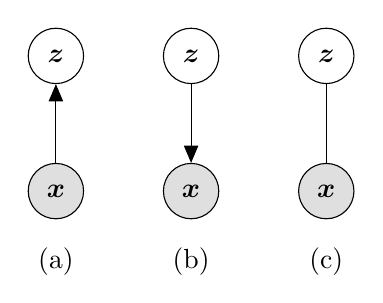
\begin{tikzpicture}

% Define nodes

\node[latent]                (zenc) {$\z$};
\node[obs, below=of zenc]                (xenc) {$\x$};

\node[latent, right=of zenc]               (zdec) {$\z$};
\node[obs, below=of zdec]                (xdec) {$\x$};

\node[latent, right=of zdec]             (z) {$\z$};
\node[obs, below=of z]                   (x) {$\x$};

 \node[const, below=of xenc, yshift=0.65cm]  {(a)} ; %
 \node[const, below=of xdec, yshift=0.65cm]  {(b)} ; %
 \node[const, below=of x, yshift=0.65cm]  {(c)} ; %

% Connect the nodes
\edge [-] {x} {z} ; %
\edge [bend left] {xenc} {zenc} ; %
\edge [bend left] {zdec} {xdec} ; %

\end{tikzpicture}
    \caption{A \MIM model learns two factorizations of a joint distribution.
    (a) Encoding factorization. (b) Decoding factorization.
    (c) The estimated joint distribution.
    % (undirected graphical model).
    }
    \label{fig:mim-model}
% \end{wrapfigure}
\end{figure}

Our goal is to find a consistent encoder-decoder pair, representing a joint
distribution over the observation and latent domains, with high mutual
information between observations and latent states. By consistent, we mean 
that the encoding and decoding distributions $\Menc(\z | \x)\, \pjoint(\x)$ 
and $\Mdec(\x | \z)\, \pjoint(\z)$, define the same joint distribution.
Figure \ref{fig:mim-model} depicts this basic idea, in which the distribution is
valid and identical under both the encoding and decoding distributions, and is, in a
sense, an undirected model with two valid factorizations.  We note that consistency 
is achievable in the VAE when the approximate posterior $\Menc(\z | \x)$ is capable 
of representing the posterior under the decoding distribution $\Mdec(\z | \x)$.
In the general case, however, consistency is not usually achieved.

In contrast to the asymmetric divergence between encoding and decoding
distributions in the VAE objective \eqref{eq:vae-kl}, here we consider a
symmetric measure, namely, the well-known Jensen-Shannon divergence (JSD),
\begin{equation}
    \mathrm{JSD}(\params) ~=~
    \frac{1}{2}\Big( \, \DKL{\Pdec}{\Msamp} + \DKL{\Penc}{\Msamp}\, \Big) ~,
\end{equation}
where $\Msamp$ is an equally weighted mixture of the encoding
and decoding distributions; i.e.,
\begin{equation}
   \Msamp ~=~ \frac{1}{2} \big( \,\Pdec + \Penc \, \big)  ~.
   \label{eqn:msamp}
\end{equation}

Symmetry emphasizes consistency between the encoding and decoding distributions.
To learn useful latent representations we also want high mutual information 
between $x$ and $z$.
Indeed, the link between mutual information and representation learning has been explored
in many works in the literature \citep{hjelm2018learning,Hjelm2018,Chen2016}.
Here, to emphasize high mutual information, we add a particular regularizer of the form
\begin{align}
    \mathrm{R}_\mathrm{H}(\params) &= ~\frac{1}{2} \big( \, H(\Pdec) + H(\Penc) \, \big) 
    ~ .
    \label{eq:mi-regularizer}
\end{align}
This is the average of the joint entropy over $\x$ and $\z$ according
to the encoding and decoding distributions. This is related to mutual
information by the identity $H(\x, \z) = H(\x) + H(\z) - I(\x; \z)$.
That is, minimizing joint entropy encourages the minimization of the marginal entropy
and maximization of the mutual information. 
In addition to encouraging high mutual information, one can show that this
particular regularizer has a deep connection to JSD and entropy of $\Msamp$, i.e., 
\begin{equation}
    \mathrm{JSD}(\params) + \mathrm{R}_\mathrm{H}(\params) ~=~ H(\Msamp) ~.
    \label{eq:jsd-h}
\end{equation}
The derivation for Equation \eqref{eq:jsd-h} is
given in the supplementary material.


\section{Mutual Information Machine}
\label{sec:mim}

Section \ref{sec:symmetry_and_mutual_information} formulates a loss function
\eqref{eq:jsd-h} that reflects our desire for model symmetry and high mutual information.
This objective is difficult to optimize directly since we do not know how to evaluate 
$\log\pjoint(\x)$ in the general case (\ie, we do not have an exact closed-form 
expression for $\pjoint(\x)$).
As a consequence, we introduce parameterized approximate priors, $\Menc(\x)$ and $\Mdec(\z)$,
to derive tractable bounds on the penalized Jensen-Shannon divergence.
This is similar in spirit to VAEs, which introduce a parameterized approximate posterior.
These parameterized priors, together with the conditional encoder and decoder,
$\Menc(\z | \x)$ and $\Mdec(\x | \z)$, comprise a new pair of joint distributions,
\begin{align*}
    \Menc (\x, \z ) & \equiv \Menc\left(\z| \x\right) \Menc\left(\x\right) \\
    \Mdec (\x, \z ) & \equiv \Mdec\left(\x| \z\right) \Mdec\left(\z\right)  ~.
\end{align*}

These new joint distributions allow us to formulate a new, tractable loss
that bounds $H(\Msamp)$:
% \begin{align*}
%     \CEloss(\params)~ &\equiv ~H(\Msamp, \Mmodel) \\
%     &= ~\DKL{\Msamp}{\Mmodel} + H(\Msamp) \\
%     &\geq ~H(\Msamp)
%     %% \MIMloss(\params) &\equiv \frac{1}{2} ( H(\Msamp, \Menc \left(\x, \z \right)) + H(\Msamp, \Mdec \left(\x, \z \right)))
% \end{align*}
\begin{eqnarray}
    \CEloss(\params)
    &\equiv& H(\Msamp, \Mmodel)   \nonumber \\
    &=&  \DKL{\Msamp}{\Mmodel} + H(\Msamp) \nonumber \\
    &\geq&  H(\Msamp) ~,
    \label{eq:LCE}
\end{eqnarray}
where $H(\Msamp, \Mmodel)$ denotes the cross-entropy between $\Msamp$ and $\Mmodel$,
and
\begin{equation}
    \Mmodel ~= ~ \frac{1}{2} \big( \, \Mdecjoint + \Mencjoint \, \big) ~.
\end{equation}
In what follows we refer to $\CEloss$ as the cross-entropy loss.
% In what follows we refer to $\CEloss$ as the cross entropy loss,
% and $\MIMloss$ as the mutual information machine (MIM) loss.
It aims to match the model prior distributions to the anchors, while also
minimizing $H(\Msamp)$. The main advantage of this formulation is that the
cross-entropy loss can be trained by Monte Carlo sampling from the anchor
distributions with the reparameterization trick~\citep{Kingma2013, Rezende2014}.

At this stage it might seem odd to introduce a parametric prior for $\pjoint(\z)$.
Indeed, setting it directly is certainly an option.
Nevertheless, in order to achieve consistency between $\Mdecjoint$ and $\Mencjoint$
it can be advantageous to allow $\Mdec(\z)$ to vary.
Essentially, we trade-off latent prior fidelity for increased model consistency.
We give more insight in the supplementary material. \kevin{double check this}

One issue with $\CEloss$ is that, while it will try to enforce consistency
between the model and the anchored distributions, i.e.,
$\Mdec (\x, \z ) \approx \Mdec(\x | \z)\pjoint(\z)$ and
$\Menc(\x, \z) \approx \Menc(\z | \x)\pjoint(\x)$, it will not directly
try to achieve model consistency: $\Mdec (\x, \z ) \approx \Menc(\x, \z)$.
To remedy this, we bound $\CEloss$ using Jensen's inequality, \ie,
\begin{align}
    \MIMloss(\params)~ &\equiv ~\frac{1}{2}
    \big(\, H(\Msamp, \Menc \left(\x, \z \right) ) + H(\Msamp, \Mdec \left(\x, \z \right)) \, \big)
    \label{eq:mimloss}  \\
    &\geq ~\,  \CEloss(\params) ~.
    \label{eq:mim_celoss}
\end{align}

Equation \eqref{eq:mimloss} gives us the loss function for the Mutual Information 
Machine (MIM).  It is an average of cross entropy terms between the mixture 
distribution $\Msamp$ and the model encoding and decoding distributions respectively.
To see that this encourages model consistency, it can be shown that $\MIMloss$ is
equivalent to $\CEloss$ plus a non-negative model consistency regularizer; i.e.,
\begin{align}
    \MIMloss(\params) ~= ~\CEloss(\params) + \RMIM(\params) ~.
    \label{eq:LMIM-LCE}
\end{align}
The non-negativity of $\RMIM$ is a simple consequence of 
$\MIMloss(\params) \ge \CEloss(\params)$ in \eqref{eq:mim_celoss}.
One can further show (see supplementary material) that $\RMIM(\params)$ satisfies
\begin{align}
    \RMIM(\params) ~& = ~\frac{1}{2}
    \big(\,\DKL{\Msamp}{\Mdecjoint} + \DKL{\Msamp}{\Mencjoint} \big) - \DKL{\Msamp}{\Mmodel} \label{eq:RMIM-DKL}  \\
    % &= ~ \MIMloss(\params) - \CEloss(\params) \nonumber \\
    &= ~ \E{\x,\z \sim \Msamp}{-\log \, \frac{\sqrt{\Menc \left(\x, \z \right) \cdot \Mdec \left(\x, \z \right)}}{\frac{1}{2} (\Menc \left(\x, \z \right) + \Mdec \left(\x, \z \right))} } 
    ~ .
    \label{eq:RMIM}
\end{align}
% The non-negativity of $\RMIM(\params)$ also follows from the
% fact that the geometric mean is always less than or equal to the algebraic 
% mean of two non-negative quantities. 
One can conclude from \eqref{eq:RMIM} that the regularizer $\RMIM$ is zero 
only when the two joint model distributions, $\Menc \left(\x, \z \right)$
and $\Mdec \left(\x, \z \right)$, are identical under fair samples from 
the joint sample distribution $\Msamp \left(\x, \z \right)$.
In practice we find that encouraging model consistency also helps stabilize learning.

To understand the MIM objective in greater depth, we find it helpful to express $\MIMloss$ 
as a sum of fundamental terms that provide some intuition for its expected behavior.  
In particular, as derived in the supplementary material:
\begin{align}
    \MIMloss(\params)~ &=  ~
    \mathrm{R}_\mathrm{H}(\params) \, +\,
    \frac{1}{4}\big(\, \DKL{\pjoint(\z)}{ \Mdec(\z)}  + \DKL{\pjoint(\x)}{\Menc(\x)} \big)
    \nonumber \\
    & \qquad
    +\, \frac{1}{4}\big(\,\DKL{\Penc }{ \Mdec(\x, \z)} + \DKL{\Pdec}{ \Menc(\z , \x)} \big)
    \label{eq:MIM-parts}
\end{align}
The first term in \eqref{eq:MIM-parts}, as discussed above, encourages high mutual
information between observations and latent states. The second term shows that MIM
directly encourages the model prior distributions to match the anchor distributions.
Indeed, the KL term between the data anchor and the model prior is the maximum
likelihood objective.
The third term encourages consistency between the model distributions and the
anchored distributions, in effect fitting the model decoder to samples drawn from
the anchored encoder (cf.\ VAE), and, via symmetry, fitting the model encoder to
samples drawn from the model decoder (both with reparameterization).
In this view, MIM can be seen as simultaneously training and distilling a model
distribution over the data into a latent variable model.
The idea of distilling density models has been used in other domains, e.g.,
for parallelizing auto-regressive models~\citep{oord2017parallel}.

% , however to our knowledge $\MIMloss$ is
% the first objective that can train both student and teacher simultaneously under a single principled loss function.
% Kevin: Don't want to oversell, because this would imply that we should compare to their approach.

In summary, the MIM loss can be viewed as an upper bound on the entropy
of a particular mixture distribution $\Msamp$:
\begin{eqnarray}
    \MIMloss(\params) &=& 
    ~\frac{1}{2} \big(\, H(\Msamp, \Menc \left(\x, \z \right) ) + 
    H(\Msamp, \Mdec \left(\x, \z \right)) \, \big) \nonumber \\
    &=& H(\Msamp, \Mmodel) + \RMIM(\params) \nonumber  \\
    &\geq& H(\Msamp, \Mmodel) \nonumber \\
    &\geq& H(\Msamp) \nonumber  \\
    &=&  H_{\Msamp} (\x) + H_{\Msamp} (\z) - I_{\Msamp} (\x;\z) 
    \label{eq:MIM-symmetric-bound}
\end{eqnarray}
Through the MIM loss and the introduction of the parameterized model
distribution $\Mmodel$, we are pushing down on the entropy of the anchored
mixture distribution $\Msamp$, which is the sum of marginal entropies minus 
the mutual information.  Minimizing the MIM bound yields consistency of the 
model encoder and decoder, and high mutual information of $\Msamp$ between 
observations and latent states.

% The relations in Equation \eqref{eq:MIM-symmetric-bound} also offer some insight
% into the tightness of the bounds.
% The effects of minimizing $\MIMloss(\params)$ are twofold. The minimization of the
% consistency regularizer $\RMIM(\params)$ in the upper bound also directly affects
% the target objective $H(\Msamp)$, by virtue of sharing encoder and decoder parameters.
% Effectively, by shrinking the consistency gap $\RMIM(\params)$, either $\MIMloss$ minimizes the upper bound on the cross entropy $H(\Msamp, \Mmodel)$, or the entropy $H(\Msamp)$ increases the lower bound of the cross entropy.
% In other words, MIM learning is effectively changing the optimization problem (\ie, by altering $H(\Msamp)$)to be easier for the model to learn, while also changing the model to better fit the data.
% This "dual" optimization can be understood as a symmetric equivalent of the
% optimization of a single bound in VAE learning.
% \david{Still not sure I understand this fully.}
% \micha{I clarified it}
% \kevin{This might be worth talking about then. It could be helpful to consider (for our own understanding, not the paper) H(P, Q) for any P and Q where we are allowed to vary one, the other, or both.}

% The \MIM learning objective relates to MI as follows,
% \begin{align}
% I_{\Msamp} (\x;\z) -H_{\Msamp(\x)} ( \x ) -H_{\Msamp(\z)} ( \z ) ~ &  = -H_{\Msamp}( \x, \z ) \\
% & \ge  -H( \Msamp, \Mmodel ) \\
% &  \ge -\frac{1}{2} \left(H \left( \Msamp, \Menc \right)+H \left( \Msamp, \Mdec \right)\right)  \label{eq:mim-mi-lower-bound} \\
%  & = -H \left( \Msamp, \Mmodel \right) -\RMIM(\params)
% \end{align}
% where Equation \eqref{eq:mim-mi-lower-bound} is the objective in a maximization optimization problem. The above relation offers insights regarding the tightness of the lower bound. Maximizing Equation \eqref{eq:mim-mi-lower-bound} pushes up the lower bound, while simultaneously pulling down the upper bound (\ie, the upper bound shares the parametric encoder and decoder). This relation can be viewed as a student-teacher joint optimization. The lower bound improves the model $\Mmodel$ (\ie student), while the upper bound adapts the optimization problem (\ie, the teacher) in order to close the gap. This optimization process occurs concurrently with pushing both bound (lower and upper) up, as the cross entropy term $H( \Msamp, \Mmodel )$ appears in both.


% \begin{align}
% R_{\params}\left(\x,\z \right) & = \log \left(\frac{\sqrt{\Menc(\x,\z) \cdot \Mdec(\x,\z)}}{\frac{1}{2} \left( \Menc(\x,\z)+\Mdec(\x,\z) \right)}  \right) \le 0 \label{eq:mim-consistency-regularizer} \\
% \RMIM(\params)  & = -\E{\Msamp}{R_{\params}} \ge 0
% \end{align}


% \kevin{either put the figure here or refer to supplementary material.}
% \micha{I believe it is important to have the explicit relation to MI due to lower bound over entropy (either here or in the previous section). In my understanding MIM works well because it is an efficient/tractable lower bound for maximizing the MI of $\Msamp$. $\Mmodel$ is an auxiliary tool to train for encoder/decoder to do so + supporting priors to make it tractable. In the current formulation it is hidden.}

% \begin{equation}
% R_{\params}\left(\x,\z \right) = \log \left(\frac{\sqrt{\Menc(\x,\z) \cdot \Mdec(\x,\z)}}{\frac{1}{2} \left( \Menc(\x,\z)+\Mdec(\x,\z) \right)}  \right) \le 0 \label{eq:mim-consistency-regularizer}
% \end{equation}
% \begin{align}
% I_{\Msamp} (\x;\z) -H_{\Msamp(\x)} ( \x ) -H_{\Msamp(\z)} ( \z ) ~ &  = -H_{\Msamp}( \x, \z ) \\
% & \ge  -H( \Msamp, \Mmodel ) \\
% &  \ge -\frac{1}{2} \left(H \left( \Msamp, \Menc \right)+H \left( \Msamp, \Mdec \right)\right)  \\
%  & = -H \left( \Msamp, \Mmodel \right) + \E{\Msamp}{R_{\params}}
%  \label{eq:mim-mi-bound}
% \end{align}

% \micha{The stroy in my mind.
% [CONCEPTUAL]: \MIM is a tractable learning method to maximize MI of a joint distribution with anchors ($\Msamp$) and corresponding encoder and decoder. Since it hard (anchors might not have analytic form) we introduce $\Mmodel$ with auxiliary priors. The priors are there to make the learning tractable, but it turns out they are also useful by themselves.
% [INTERPRETABLE]: Breaking lower bound to interpertable expressions, and justifying CE as a loss. This allows us to design experiments, and demonstrate the mechanics of \MIM. }

\input{sections/learning}
\section{Relation to VAE and Posterior Collapse}
\label{sec:posterior-collapse}

Here, before turning to empirical results, it is useful to briefly revisit 
similarities and differences between MIM and the canonical VAE formulation. 
To that end, one can show from Equations \eqref{eq:vi-objective}
and \eqref{eq:vae-kl} that the VAE loss can be expressed in a form
that bears similarity to the MIM loss in Equation \eqref{eq:mimloss}.
In particular, following the derivation in the supplementary material,
\begin{equation}
\begin{aligned}
\VAEloss ~=~
\frac{1}{2} & \Big( \, H(\Msamp^\mathrm{VAE}, \,\Menc(\z|\x)\,\pjoint(\x))
+ H(\Msamp^\mathrm{VAE},\, \Mdec(\x|\z)\,\pjoint(\z)) \, \Big) 
\\
& ~~ - H_{\Msamp^\mathrm{VAE}}(\x) - H_{\Msamp^\mathrm{VAE}}(\z) + I_{\Msamp^\mathrm{VAE}}(\x;\z)  ~.
\label{eq:vi-as-ml-objective-text}
\end{aligned}
\end{equation}
where $\Msamp^\mathrm{VAE}(\x,\z) ~=~ \Menc(\z|\x)\, \pjoint (\x)$.
Like the MIM loss, the first term in Equation \eqref{eq:vi-as-ml-objective-text}
in the average of two cross entropy terms, between a sample distribution 
and the encoding and decoding distributions. Unlike the MIM loss, these 
terms are asymmetric as the samples are drawn only from the encoding 
distribution. Also unlike the MIM loss, the VAE loss includes the 
last three terms in Equation \eqref{eq:vi-as-ml-objective-text}, 
which the sum of which comprise the negative joint entropy $-H(\z,\x)$ 
under the sample distribution $\Msamp^\mathrm{VAE}$.

While the MIM objective explicitly encourages high mutual information 
between observations and corresponding latent embedings, this VAE loss 
includes a term that encourages a reduction in the mutual information. 
We posit that this plays a significant role in the phenomena often 
referred to as posterior collapse, in which the variance of the variational 
posterior grows large and the latent embedding conveys relatively little 
information about the observations  (e.g., see \citep{ChenKSDDSSA16} 
and others).  

%%%%%%%%%%%%%%%%%%%%%%%%%%%%%%%%%%%
% \david{old version}
% Here we discuss a possible root cause for the observed phenomena 
% of posterior collapse, and show that VAE learning can be viewed 
% as an asymmetric MIM learning with a regularizer that encourages 
% the appearance of the collapse. We further support that idea in 
% the experiments in Section\ \ref{sec:posterior-collapse-mim-vae}.
% As discussed earlier, VAE learning entails maximization of a variational lower
% bound (ELBO) on the log-marginal likelihood, or equivalently, minimization of
% Equaiton\ \eqref{eq:vae-kl}.
% To connect the loss in Equation\ \eqref{eq:vae-kl} to MIM, we manipulate it to the following form
% \begin{align}
% & \frac{1}{2} \big(\, H(\Msamp^\mathrm{VAE},\, \Mdec(\x|\z)\,\pjoint(\z))
% + H(\Msamp^\mathrm{VAE}, \,\Menc(\z|\x)\,\pjoint(\x))\, \big) + \nonumber \\
% & - H_{\Msamp^\mathrm{VAE}}(\x) - H_{\Msamp^\mathrm{VAE}}(\z) + I_{\Msamp^\mathrm{VAE}}(\x;\z)  ~.
% \label{eq:vi-as-ml-objective-text}
% \end{align}
% where $\pjoint(\x)$ is the data distribution, which is assumed to be independent of model
% parameters $\theta$ and to exist almost everywhere (i.e., complementing $\pjoint(\z)$),
% and $\Msamp^\mathrm{VAE}(\x,\z) ~=~ \pjoint (\x)\,\Menc(\z|\x)$.
% Importantly, because $\pjoint(\x)$ does not depend on $\params$, the gradients of
% Eqs.\ \eqref{eq:vi-as-ml-objective-text} and \eqref{eq:vae-kl}
% are identical up to a multiple of $\frac{1}{2}$ and an additive constant, so they share the same stationary points.
% We refer the reader to the supplementary material for detailed derivation.
% We note that $\Msamp^\mathrm{VAE}$ comprises the encoding distribution in $\Msamp$.
% The sum of the last three terms in Equation\ \eqref{eq:vi-as-ml-objective-text}
% is the negative joint entropy $-H(\z, \x)$ under the sample distribution $\Msamp^\mathrm{VAE}$.
% , i.e., $-H_{\Msamp^\mathrm{VAE}}(\z|\x )$.
%
% Equations\ \eqref{eq:vae-kl} and \eqref{eq:vi-as-ml-objective-text}, the VAE objective and 
% VAE as regularized cross entropy objective respectively, define
% equivalent optimization problems, under the assumption that  $\pjoint(\x)$ and
% samples $\x \sim \pjoint(\x)$ do not depend on the parameters $\params$, and that
% the optimization is gradient-based.
% Equation \eqref{eq:vi-as-ml-objective-text} is the average of two cross-entropy objectives (
% \ie, between sample distribution $\Msamp^\mathrm{VAE}$ and the model decoding and encoding distributions,
% respectively), along with a joint entropy term (\ie, last three terms), which can be viewed as a
% regularizer that encourages a reduction in mutual information and increased entropy in $\z$ and $\x$.
% We note that Equation \eqref{eq:vi-as-ml-objective-text} is similar to the \MIM objective in Equation \eqref{eq:mimloss},
% but with a different sample distribution, where the priors are defined to be the anchors, and with an additional regularizers.
% In other words, Equation\ \eqref{eq:vi-as-ml-objective-text} suggests that VAE learning
% implicitly encourages lower mutual information, which can manifest itself in collapsing some of the dimensions
% of the posterior to hold little or no information (\ie, match the prior), and poor reconstruciton (\eg, blurry images).
% This runs contrary to the goal of learning useful latent representations, and we
% posit that it is an underlying root cause for {\em posterior collapse}, 
% \david{not sure this is the definition we want.} 
% wherein the encoder matches the prior and thus provides weak information about the latent state
% % , so the decoder effectively becomes trained to match the prior
% (e.g., see \citep{ChenKSDDSSA16} and others).

\section{Experiments} \label{sec:experiments}

In what follows we empirically probe properties of the MIM model,
with the VAE as a baseline.  We consider both low-dimensional synthetic 
datasets and well-known images datasets, including MNIST \cite{LeCun1998}, 
Fashion MNIST \cite{DBLP:journals/corr/abs-1708-07747} and Omniglot \cite{Lake2015}. 
The code used to generate the results reported below is available 
from \href{https://github.com/seraphlabs-ca/MIM}{https://github.com/seraphlabs-ca/MIM}.
In all experiments (unless otherwise specified) we use Adam optimizer \cite{2014arXiv1412.6980K} with $lr = 1e-3$, and
mini-batch of size 128. We stopped training for all experiments when validation loss
has not improved for 10 epochs.

%%%%%%%%%%%%%%%%%%%%%%%%%%%%%%%%%%%%%%%%%%%%%%%%%%%%%%%%
\subsection{2D Mixture Model Data} 
\label{sec:posterior-collapse-mim-vae}


We begin with a synthetic dataset of 2D observations $\x \in \mathbb{R}^2$
and a 2D latent space, $\z \in \mathbb{R}^2$. In two dimensions we can easily 
visualize the model and measure quantitative properties of interest (\eg, mutual information).
Data are drawn from a Gaussian mixture model with five isotropic components
with standard deviation 0.25; the black contours in Fig.\ \ref{fig:posterior-collapse-qualitative} (top) depict level sets of constant density $\pjoint(\x)$. 
The latent anchor (bottom), $\pjoint(\z)$, is an isotropic standard normal distribution.
The encoder and decoder conditional distributions are Gaussian, the means
and variances of which are regressed from the input using two fully 
connected layers and swish activation \cite{Ramachandran2017}).
Finally, the parameterized data prior, $\Menc(\x)$, is defined to be the 
marginal of the decoding distribution \eqref{eqn:q-marginal}, so
the only model parameters are those of the encoder and decoder.
As such we can learn models with MIM and VAE objective that share
the same architectures and parameterizations.

Figure \ref{fig:posterior-collapse-qualitative} depicts three models 
for the VAE (even columns) and MIM (odd columns), with increasing numbers 
of hidden units (moving left to right) to control model expressiveness.
The top row (for VAE and MIM respectively) depict observation 
space where black contours are levels sets of constant density 
$\pjoint (\x)$, and red points are reconstructed samples, 
i.e., one point drawn from the decoder $\Mdec(\x | \z' )$ where $\z'$ is 
drawn from the encoder $ \Menc(\z' | \x') $, given observation $\x'$ 
from $\pjoint(\x)$ in the test set.
With each case we also report the mutual information and the root-mean-squared,
with MIM showing a superior performance.


\begin{figure}[t]
    \centering
    \setlength{\tabcolsep}{0pt}
    \begin{tabular}{*6{>{\centering\arraybackslash}m{0.167\textwidth}}}
      {\scriptsize VAE} & {\scriptsize MIM} & {\scriptsize VAE} & {\scriptsize MIM} & {\scriptsize VAE} & {\scriptsize MIM} \\
      \includegraphics[width=0.165\columnwidth]{images/vae-as-mim-toy-2d/toy4/plots/vae_logvar10_mid-dim5_layers2_q-x0marginal_q-zx0_p-z0anchor_p-xz0/reconstruction_best.png}
    & \includegraphics[width=0.165\columnwidth]{images/vae-as-mim-toy-2d/toy4/plots/mim-samp_logvar10_mid-dim5_layers2_q-x0marginal_q-zx0_p-z0anchor_p-xz0/reconstruction_best.png}
    & \includegraphics[width=0.165\columnwidth]{images/vae-as-mim-toy-2d/toy4/plots/vae_logvar10_mid-dim20_layers2_q-x0marginal_q-zx0_p-z0anchor_p-xz0/reconstruction_best.png}
    & \includegraphics[width=0.165\columnwidth]{images/vae-as-mim-toy-2d/toy4/plots/mim-samp_logvar10_mid-dim20_layers2_q-x0marginal_q-zx0_p-z0anchor_p-xz0/reconstruction_best.png}
    & \includegraphics[width=0.165\columnwidth]{images/vae-as-mim-toy-2d/toy4/plots/vae_logvar10_mid-dim500_layers2_q-x0marginal_q-zx0_p-z0anchor_p-xz0/reconstruction_best.png}
    & \includegraphics[width=0.165\columnwidth]{images/vae-as-mim-toy-2d/toy4/plots/mim-samp_logvar10_mid-dim500_layers2_q-x0marginal_q-zx0_p-z0anchor_p-xz0/reconstruction_best.png}
    \\
    \multicolumn{2}{c}{(a) $h \in \mathbb{R}^{5}$ } & \multicolumn{2}{c}{(b) $h \in \mathbb{R}^{20}$ } & \multicolumn{2}{c}{(c) $h \in \mathbb{R}^{500}$ } \\
    \end{tabular}
    \caption{
    VAE and MIM models with 2D inputs, a 2D latent space, and 5, 20 and 500 hidden units. 
    Top row: Black contours depict level sets of $\pjoint(\x)$, red points are 
    reconstructed test points.
    Bottom row: Green contours are one standard deviation ellipses of 
    $\Menc(\z|\x)$ for test points. Dashed black circles depict one standard 
    deviation of $\pjoint (\z)$.
    (a) For weak architectures MIM and VAE exhibit high posterior variance.
    (b,c) For more expressive architectures the VAE predictive variance remains high,
    an indication of posterior collapse.
    MIM generally produces lower predictive variance and lower reconstruction 
    errors, consistent with high mutual information (see inset quantities).
    }\label{fig:posterior-collapse-qualitative}
\end{figure}

\begin{figure}[ht]
    \centering
    \setlength{\tabcolsep}{0pt}
    \begin{tabular}{*4{>{\centering\arraybackslash}m{0.25\textwidth}}}
      \includegraphics[width=0.24\columnwidth]{{images/vae-as-mim-toy-2d/toy4/stats/fig.MI_ksg}.png}
    & \includegraphics[width=0.24\columnwidth]{{images/vae-as-mim-toy-2d/toy4/stats/fig.H_q_x.symlog}.png}
    & \includegraphics[width=0.24\columnwidth]{{images/vae-as-mim-toy-2d/toy4/stats/fig.x_recon_err.symlog}.png}
    & \includegraphics[width=0.24\columnwidth]{{images/vae-as-mim-toy-2d/toy4/stats/fig.clf_acc_KNN5}.png}
    \\
    (a) MI & (b)  $\E{\x \sim \pjoint(\x)}{\log \Menc(\x)}$ & (c) Recon.\ Error & (d) Classif.\ (5-NN)
    \end{tabular}
    \caption{Test performance for MIM (blue) and VAE (red) for 2D GMM experiment,
    all as functions of the number of hidden units (on x-axis), based on 10 learned
    models in each case. From left to right, plots show mutual information, log marginal 
    probability of test points, reconstruction error, and k-NN classification performance.
    \david{for these plots: link dots with lines, and on x-axis perhaps only label 20, 100, 
    200, 300, 400, and 500. Simpler format. Stdev bars or min-max?}\micha{will do. stdev in all plots}
    }\label{fig:posterior-collapse-quantitative}
\end{figure}


Bottom row of Fig.\ \ref{fig:posterior-collapse-qualitative}
depict the latent space behavior.  The dashed black circle 
depicts one standard deviation of $\pjoint(\z)$. Each green 
curve depicts a one standard deviation ellipse of the encoder posterior  
$\Menc(\z' | \x')$ for a data point $\x'$ drawn from $\pjoint(\x)$.
One can clearly see that for the weakest architecture, with only 5 
hidden units, both MIM and VAE posteriors have large variances.
When the number of hidden units increases to 20, however, it is 
clear that will the VAE posterior variance remains very large in
one dimension, the MIM encoder produces much tighter posteriors 
densities.  Even with more a expressive architecture, VAE posteriors depict
continue to exhibit very high variances, a common sign of posterior collapse. 



To quantify this behavior for each architecture in  
Fig.\ \ref{fig:posterior-collapse-qualitative}, Fig.\ 
\ref{fig:posterior-collapse-quantitative} plots the mutual information, 
the average log marginal of test points under the model $\Menc$,
the reconstruction error of test points, and 5-NN classification
(predicting which of five GMM components the test points were drawn from).
Following  \cite{Hjelm2018}, we estimate mutual information 
using the KSG mutual information estimator \cite{PhysRevE.69.066138,DBLP:journals/corr/GaoOV16},  
based on a K-NN neighborhoods with $k=5$, and measure the quality of the representation with classification axuliary task.

One can see that mutual information and the average log likelihood 
of the test data under the MIM model are higher than for VAE models.
One can also see that mutual information saturates for MIM as the
number of hidden units grow larger than 20.
(We direct the reader to Sec.\ \ref{sec:entropy-as-mi-regularizer}
of the supplementary material for experiments on variants of 
MIM and VAE tease apart the impact of specific terms of the 
respective objectives.)

One can also see from Fig.\ \ref{fig:posterior-collapse-qualitative} that as the models 
becomes sufficiently expressive, in terms of the number of 
hidden units, the MIM encoding variance becomes extremely small,
and the reconstruction error in Fig.\ \ref{fig:posterior-collapse-quantitative} approaches 0.
Effectively, the encoder and decoder learn an (approximately) invertible mapping using 
an unconstrained architecture (demonstrated here for the 2D case), when the 
dimensionality of the latent representation and the observations is the same.

The VAE, by comparison, is prone to posterior collapse, with latent embeddings 
with relatively low mutual information. In regard, we note that several 
papers have described ways to mitigate posterior collapse in VAE learning, e.g., 
by lower bounding, or annealing the KL divergence term in the VAE objective 
(e.g., \citep{DBLP:journals/corr/abs-1711-00464,DBLP:journals/corr/abs-1901-03416}), 
or by limiting the expressiveness of the decoder (e.g., \citep{ChenKSDDSSA16}).
We posit that MIM does not suffer from this problem as a consequence of 
the objective design principles that encourage high mutual information
between observations and the latent representation.


\section{Related Work}
\label{sec:related-work}

The VAE \cite{Kingma2013} is a latent variable model (LVM) that is widely used in learning a useful latent representation.
Typically, the quality of the learned representation is measured by auxiliary tasks such as classification \cite{DBLP:journals/corr/BengioTPPB17}.
The VAE also provides a remarkable sampling capability (\eg, \cite{DBLP:journals/corr/abs-1901-03416}) which is considered as an evidence for 
the quality of the learned representation. Unfortunately, it has been observed that a powerful decoder
can suffer from posterior collapse \citep{DBLP:journals/corr/BowmanVVDJB15,ChenKSDDSSA16,
DBLP:journals/corr/abs-1901-03416,DBLP:journals/corr/OordKK16,
DBLP:journals/corr/abs-1711-00937}. where such a decoder ignores the encoder in some dimensions, 
and the learned representation has low mutual information with the observations.
While several methods has been proposed to mitigate the problem \cite{DBLP:journals/corr/abs-1711-00464, DBLP:journals/corr/abs-1901-03416}, no root cause has been suggested to date.

In addition, mutual information has been used to measure the quality of the representation \cite{Hjelm2018,hjelm2018learning}. Mutual information, together with disentanglement, are considered as corner stones 
of a useful representation. Normalizing flows \cite{Rezende2015,Dinh2014,Dinh2016a,Kingma2018,DBLP:journals/corr/abs-1902-00275} directly maximizes mutual information
by restricting the architecture to be invertible and tractable. This, however, requires the latent dimension to be the same as the dimension of the observations (\ie, no bottleneck).
As a result no information is lost, and thus normalizing flows cannot be used in order to learn a concise representation of high dimensional data (\eg, images). Here, MIM can be viewed as a generalization of invertibility, which supports change of dimensionality, and behaves as an invertible model when dimensionality is the same.

A closer formulation to \MIM is proposed in \cite{DBLP:journals/corr/BornscheinSFB15}, which shares several of the design
principles with our work, including symmetry (\ie, consistency of encoding and decoding distributions). 
One importance difference however, is that the formulation proposed in \cite{DBLP:journals/corr/BornscheinSFB15} advocates for a joint density
in terms of the geometric mean between the encoder and decoder, for which they have to 
compute the partition function.  As a result the model learning is computationally very expensive.

Alternatively,  GANs \cite{NIPS2014_5423}, which for the most part focus on decoder properties without a proper inference model,
has been shown to minimize JSD between the observations anchor $\pjoint(\x)$ and the model generative process $\Menc(\x)$ (\ie, the marginal of the decoding distribution in \MIM terms). 
In particular, \citep{DonahueKD16-BiGAN,Bang-BiGAN2018} recognizes the importance of symmetry in learning generative models with reference to symmetric discriminators on $x$ and $z$. In contrast, here we target JSD between the joint encoding and decoding distributions, together with a regularizer to encourage high mutual information within a consistent model.


\section{Discussion and Conclusions} \label{sec:conclusion}


We introduce a new representation learning framework, named the {\em mutual information machine} (MIM), that defines a generative model which directly targets high mutual information (\ie, between the observations and the latent representation), and symmetry (\ie, consistency of encoding and decoding factorizations of the joint distribution). We derive a variational upper bound that enables the maximizion of mutual information in the learned representation for high dimensional continuous data, without the need to directly compute it. We then provide a possible explanation for the phenomena of posterior collapse, demonstrate  its validity, and show that MIM does not suffer from it. We also provide a comparison to VAE, and demonstrate that MIM learning leads to higher mutual information, and better clustering in the latent representation, for the same parametrization of the model. 

In addition, we show that MIM behaves similar to a deterministic autoencoder when the dimensionality of the latent representation is equal to that of the observations, which effectively provides invertibility via deterministic encoder-decoder. Such behaviour allows for training of invertible functions without any constraint on the architecture. Furthermore, it allows to generalize invertibility when the dimensionality differs with a probabilistic invertibility that is defined through consistency and high mutual information.

Two open questions that were not addressed in this paper: how to utilize a high capacity generative model with clustered latent representation? What is the significance of symmetry (multiple factorizations of the same distribution)? We leave that discussion for future work, where we will introduce the concept of "knowledge" - binary partition of the latent representation around areas of interest in the latent representation.


\bibliography{paper}
\bibliographystyle{plainnat}

\newpage
\appendix
\input{sections/supplementary-material}

\end{document}
